\documentclass[10pt,fleqn]{article} % Default font size and left-justified equations
\usepackage{import}
\usepackage[%
    pdftitle={Energie et puissance d'un smartphone},
    pdfauthor={Geoffrey Vaquette}]{hyperref}
\subimport{../../../../style/}{preambule}
%\fichetrue
\fichefalse

\proftrue
%\proffalse

\tdtrue
%\tdfalse

\courstrue
%\coursfalse

\subimport{../../../../style/}{new_style}
\subimport{../../../../style/}{macros_SII}
\subimport{../../../../style/}{preambule_trou}

\usepackage{siunitx}
% -------------------------------------
% Déclaration des titres
% -------------------------------------

\def\discipline{Enseignement \\Technologique \\ Transversal}
\def\xxtete{Enseignement Technologique Transversal}

\def\classe{1 STI2D}
\def\xxnumpartie{Séquence 2}
\def\xxpartie{Energie électrique et puissance d'un smartphone}

\def\xxnumchapitre{Séance 3}
\def\xxchapitre{\hspace{.12cm} Énergies, Puissances et rendement}

\def\xxposongletx{2}
\def\xxposonglettext{1.45}
\def\xxposonglety{23}
\def\xxonglet{Seq. 2 -- DS 3}

\def\xxactivite{DS}
\def\xxauteur{\textsl{Geoffrey Vaquette}}

\def\xxcompetences{%
\textsl{%
\textbf{Savoirs et compétences :}
\begin{itemize}[label=\ding{112},font=\color{ocre}]
\item CO2.1	Identifier les flux et la forme de l'énergie, caractériser ses transformations et/ou modulations et estimer l'efficacité globale d'un système.
\end{itemize}
%
}}

\def\xxfigures{
\begin{center}

\includegraphics[height=4cm]{images/smartphone.png} \\
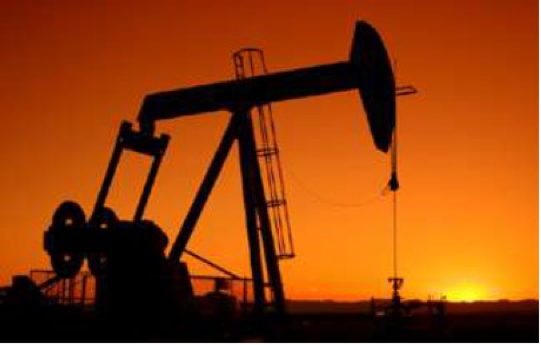
\includegraphics[height=4cm]{images/petrole.png} \\
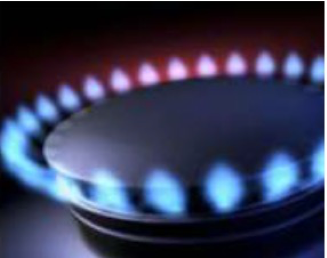
\includegraphics[height=4cm]{images/gaz.png} \\
\end{center}
}%figues de la page de garde
\def\xxpied{%
Energies, Puissances et Rendement \xxactivite%
}

%---------------------------------------------------------------------------

\renewcommand{\RemplirTrou}{true}
\begin{document}
\chapterimage{png/Fond_solaire}

\begin{obj}
Déterminer l’énergie et la puissance disponibles dans un système

L’étude suivante concerne un smartphone.

Vous serez amené-e à
 calculer l’énergie présente dans la batterie de ce téléphone ainsi que les puissances et énergies nécessaires
 nécessaires pour différentes utilisations de celui-ci.

\end{obj}
\section{Étude énergétique d'un Samsung Galaxy S9}
\subsection{Quelques données}
Caractéristiques de la batterie :
\begin{itemize}
 \item Technologie : Li-Ion (lithium-ion)
\item Capacité : $ C = \SI{3000}{mAh} $
\item Tension : $U=\SI{4.4}{V}$
\item Autonomie en utilisation : 11h et 15 min
\end{itemize}



\begin{exercise}~

\begin{question}
  Quelle solution permet de remplir la fonction « Alimenter / Stocker » dans le cas de ce smartphone ?
\end{question}
\begin{solution}
  La fonction alimenter/stocker est réalisée par la batterie du smartphone.
\end{solution}

\begin{question}
  Calculer l’énergie électrique $\omega_\text{bat}$que contient la batterie.
\end{question}
\begin{solution}
  On connaît la tension de la batterie, ainsi que sa capacité. L'énergie
  contenue dans la batterie est $$\omega_\text{bat} = U\times C = 4.4 \times \num{3000e-3}=\SI{13.2}{Wh} $$
\end{solution}

\begin{question}
  A partir des données annoncées, calculer la puissance de ce Smartphone en
 utilisation
\end{question}
\begin{solution}
La puissance moyenne est l'énergie consommé divisée par le temps qu'il a fallu pour consommer cette énergie : $P = \frac{\omega_\text{bat}}{t}$
$$P_{\text{utilisation}} = \frac{13.2}{11.4} = \SI{1.17}{W}$$
\end{solution}

\begin{question}
  En déduire le courant consommé en utilisation.
\end{question}
\begin{solution}
  Connaissant la relation liant la puissance, le courant et la tension
  $P=U\times I$, on déduit $I = \frac{P}{U}$.
  $$I_{\text{utilisation}} = \frac{1.17}{4.4} = \SI{266}{mA}$$
\end{solution}

\begin{question}
  En supposant qu’une charge complète de la batterie doit être effectuée tous les jours, déterminer l’énergie électrique $E_{\text{tel annuel}}$ consommée par le téléphone en une année.
\end{question}
\begin{solution}
  Tous les jours, le Smartphone consomme une énergie de 13.2 Wh.
Il faudra le recharger 365 fois en un an.
$$E_{\text{tel annuel}} = 365 x 13.2 = \SI{4 818}{Wh} = \SI{4.818}{kWh}$$
\end{solution}

\begin{question}
  En supposant le rendement d'un chargeur de téléphone de $\eta = 0.95$, calculez l'énergie annuelle consommée sur le réseau par un téléphone en France.

  On rappelle que $E_s = \eta \times E_e$ avec $\eta$ le rendement, $E_s$ l'énergie en \textbf{sortie} d'un système et $E_e$ l'énergie en \textbf{entrée} d'un système.
\end{question}
\begin{solution}
  On cherche l'énergie $E_{\text{elec}}$ en entrée du chargeur (nécessaire à recharger le téléphone) en connaissant l'énergie en sortie (énergie consommée par le téléphone). On a donc $ E_{\text{elec}} = \frac{E_{\text{tel annuel}}}{\eta} = \SI{5071}{Wh}$
\end{solution}

\begin{question}
Calculez l'énergie perdue (énergie non-utile) annuellement pour la recharge de téléphones portables. Sous quelle forme est perdue cette énergie ?
\end{question}
\begin{solution}
  Cette énergie est perdue sous forme de chaleur. On perd $E_{\text{perdue}} = E_{\text{elec}} * (1-\eta) $
\end{solution}

\begin{question}
  Les statistiques indiquent qu'en 2017, 73\% des français de plus de 12 ans possédaient un smartphone. En supposant que tous les français ait un portable équivalent au Galaxy S9 en consommation d'énergie, Calculez l'énergie totale que représente la recharge des téléphone en France, en 2017.
  \textit{On suppose que 59 Millions de Français avaient plus de 12 ans en 2017. }
\end{question}
\begin{solution}
  $E_{totale} = \num{59e6}\times 0.73 \times E_{elec}  = \SI{218}{GWh}$
\end{solution}

\begin{question}
Convertissez cette dernière valeur en joules (J) et en Tep. Rappel : $\SI{1}{Tep} = \SI{4.187e10}{J}$
\end{question}
\begin{solution}
  En joules : On divise le résultat en Wh par 3600

  En Tep : On divise le résultat en J par \num{4.187e10}
\end{solution}
\end{exercise}


\end{document}
